\documentclass[10pt,a4paper,twoside]{report}
\usepackage[utf8]{inputenc}

\usepackage[]{feupteses}
%\usepackage[square,sort,comma,numbers]{natbib}


\usepackage[english]{babel}


%\bibliographystyle{IEEEtran}

%\usepackage[square]{natbib}
\usepackage{graphicx}
\usepackage{framed}
\usepackage{multirow}
\usepackage{lipsum}  
\usepackage{verbatim}
\usepackage{amsmath}
\usepackage{longtable}
\usepackage{caption}
\usepackage{subcaption}


\usepackage{array}
\usepackage{adjustbox}


%\usepackage[oneside,width=17.5cm,height=24cm,left=2cm]{geometry}
%\usepackage[nolist,nohyperlinks]{acronym}

\usepackage[]{nomencl}
\usepackage[final]{pdfpages}

%\usepackage{biblatex}
%\addbibresource{references.bib}



\newcolumntype{L}[1]{>{\raggedright\let\newline\\\arraybackslash\hspace{0pt}}m{#1}}
\newcolumntype{C}[1]{>{\centering\let\newline\\\arraybackslash\hspace{0pt}}m{#1}}
\newcolumntype{R}[1]{>{\raggedleft\let\newline\\\arraybackslash\hspace{0pt}}m{#1}}

%%%  para ter capítulos xpto
%%%  https://hstuart.dk/2007/05/21/styling-the-chapter/


\usepackage{tikz, blindtext}
\usepackage{kpfonts}
\usepackage[explicit]{titlesec}
\usepackage{xcolor}
\definecolor{FEUP_color}{RGB}{140,45,25}

\newcommand*\chapterlabel{}
\titleformat{\chapter}
{\gdef\chapterlabel{}
	\normalfont\sffamily\huge\bfseries\scshape}
{\gdef\chapterlabel{\thechapter\ }}{0pt}
{\begin{tikzpicture}[remember picture,overlay]
	\node[yshift=-6cm] at (current page.north west)
	{\begin{tikzpicture}[remember picture, overlay]
		%\draw[fill=white] (-1,0) rectangle
	%	(1.2\paperwidth,8cm);
		\node[anchor=west,xshift=3cm,rectangle,
		rounded corners=1pt,inner sep=11pt,
		fill=black]
		{\color{white}\chapterlabel#1};
		\end{tikzpicture}
	};
\end{tikzpicture}
}
\titlespacing*{\chapter}{0pt}{50pt}{50pt}

\makenomenclature
\nomenclature{\textbf{AMI}}{Advanced Metering Infrastructure }
\nomenclature{\textbf{EMS}}{Energy Management System}
\nomenclature{\textbf{EIS}}{Energy Information Systems}
\nomenclature{\textbf{SG}}{Smart Grid}
\nomenclature{\textbf{IT}}{Information Technology}
\nomenclature{\textbf{AMR}}{Automatic Meter Readers}
\nomenclature{\textbf{SM}}{Smart Meter}
\nomenclature{\textbf{IEC}}{International Electrotechnical Commission}
\nomenclature{\textbf{EC}}{European Commission}
\nomenclature{\textbf{EU}}{European Union}
\nomenclature{\textbf{EGs}}{Expert Groups}
\nomenclature{\textbf{TSOs}}{Transmission System Operators}
\nomenclature{\textbf{DSOs}}{Distribution System Operators}
\nomenclature{\textbf{DNOs}}{Distribution Network Operators}

%2.2 to 2.6

\nomenclature{\textbf{WAN}}{Wide Area Network}
\nomenclature{\textbf{NAN}}{Neighborhood Area Network}
\nomenclature{\textbf{LAN}}{Local Area Network}
\nomenclature{\textbf{HAN}}{Home Area Network}
\nomenclature{\textbf{MAN}}{Metropolitan Area Network}
\nomenclature{\textbf{PEVs}}{Plug-in Electric Vehicles}
\nomenclature{\textbf{IHD}}{In-Home Displays}
\nomenclature{\textbf{MDMS}}{Meter Data Management System}
\nomenclature{\textbf{DR}}{Demand-Response}
\nomenclature{\textbf{SEIS}}{Smart Energy Management Systems}
\nomenclature{\textbf{ICT}}{Information and Communication Technologies}
\nomenclature{\textbf{O\&M}}{Operation and Management}
\nomenclature{\textbf{S2R}}{Shift2Rail program}
\nomenclature{\textbf{IP3}}{Innovation Programme 3 (of Shift2Rail)}
\nomenclature{\textbf{ODM}}{Operational Data Management}
\nomenclature{\textbf{UA}}{User Applications}
\nomenclature{\textbf{RDERMS}}{Railway dedicated Distributed Energy Resource Management System}

%chapter 3

\nomenclature{\textbf{SCADA}}{Supervisory Control and Data Acquisition}
\nomenclature{\textbf{PLC}}{Power Line Communication}
\nomenclature{\textbf{DCM}}{Data Collection Mechanism}
\nomenclature{\textbf{ADSL}}{Asymmetric  Digital  Subscriber  Line}
\nomenclature{\textbf{GSM}}{Global Systems Network}

\nomenclature{\textbf{SMS}}{Short Message Service}
\nomenclature{\textbf{CDMA}}{Code Division Multiple Access}
\nomenclature{\textbf{D-AMPS}}{Digital Advanced Mobile Phone Service}
\nomenclature{\textbf{RF}}{Radio Frequency}
\nomenclature{\textbf{WLAN}}{Wireless Local Area Network}
\nomenclature{\textbf{GPRS}}{General Packet Radio Service}
\nomenclature{\textbf{WiMAX}}{Worldwide Interoperability for Microwave Access}
\nomenclature{\textbf{IEEE}}{Institute of Electrical and Electronics Engineers}

\nomenclature{\textbf{ISO}}{International Organization for Standardization}
\nomenclature{\textbf{MAC}}{Media Access Control}
\nomenclature{\textbf{PHY}}{Physical Layer}
\nomenclature{\textbf{RFID}}{Radio Frequency Identification Devices}
\nomenclature{\textbf{ISM}}{Industrial, Scientific and Medical}
\nomenclature{\textbf{DSSS}}{Direct Sequence Spread Spectrum}

\nomenclature{\textbf{DASH7}}{Developers Alliance For Standards Harmonization of ISO 18000-7}
\nomenclature{\textbf{OFDM}}{Orthogonal Frequency-Division Multiplexing}
\nomenclature{\textbf{GMSK}}{Gaussian Minimum-Shift Keying}
\nomenclature{\textbf{LTE}}{Long Term Evolution}
\nomenclature{\textbf{QoS}}{Quality of Service}
\nomenclature{\textbf{BACnet}}{Building Automation and Control NETworks}

\nomenclature{\textbf{VSCP}}{Very Simple Control Protocol}
\nomenclature{\textbf{VSCP}}{Doctor of Philosophy}

\nomenclature{\textbf{ }}{ }
\nomenclature{\textbf{ }}{ }
\nomenclature{\textbf{ }}{ }







%some macro definitions

% format
\newcommand{\class}[1]{{\normalfont\slshape #1\/}}

% entities
\newcommand{\Feup}{Faculdade de Engenharia da Universidade do Porto}

\newcommand{\svg}{\class{SVG}}
\newcommand{\scada}{\class{SCADA}}
\newcommand{\scadadms}{\class{SCADA/DMS}}


\begin{document}

%%----------------------------------------
%% Information about the work
%%----------------------------------------
\title{Monitoring PV power converters using Wireless Sensor Networks
	\\--- \\
	Activity report}

\author{Vítor A. Morais}

%% Uncomment next line if necessary for degree
\degree{Programa Doutoral em Engenharia Electrotécnica e de Computadores}

%% Uncomment next line for date of submission
%\thesisdate{July 31, 2016}

%% Uncomment next line for copyright text
%\copyrightnotice{Name of the Author, 2016}

\supervisor{Supervisor}{António P. Martins}

%% Uncomment next line if necessary
%\supervisor{Second Supervisor}{Name of the Supervisor}

%% Uncomment committee stuff in the final version if used
%\committeetext{Approved by \ldots:}
%\committeemember{President}{Name of the President}
%\committeemember{Referee}{Name of the Referee}
%\committeemember{Referee}{Name of the Referee}

%% Uncomment signature line in the final on paper version if used
%\signature

%% Specify cover logo (in folder ``figures'')
\logo{figures/uporto.pdf}

%% Uncomment next line for additional text below the author's name (front page)
\additionalfronttext{DELIVERY VERSION}



%\chapter*{Abstract}
%Abstract goes here
%%
%%   Section 
%%
\begin{Prolog}
\cleardoublepage

\tableofcontents


%\printnomenclature

%\chapter*{Symbols}
%\begin{flushleft}

\begin{tabular}{l p{0.8\linewidth}}


kbps     & Kilobit per second (often used kbit/s or kb/s) - bit rate\\
Mbps     & Megabit per second (often used Mbit/s or Mb/s) - bit rate\\
Gbps     & Gigabit per second (often used Gbit/s or Gb/s) - bit rate\\
dB       & Decibel - Gain/Attenuation\\
kHz      & Kilohertz - Frequency\\
MHz      & Megahertz - Frequency\\
GHz      & Gigahertz - Frequency\\
km       & Kilometer - Distance\\
min      & Minute - Time\\


\end{tabular}
\end{flushleft}

	
\end{Prolog}

\StartBody

\chapter{Introduction}
%\lipsum[4-4]
This chapter presents the context, motivation and document structure of the activity report of the work "monitoring photovoltaic power converters using Wireless Sensor Networks". 

\section{Context and motivation of PhD}

The railway system is responsible for 1.3\% of entire European energy consumption, \cite{iea-uic2016}. 
The discussion of the energy efficiency in railways is a grown topic due to its contribution to the global energy consumption.

The energy efficiency analysis and management requires a detailed mapping of the energy consumption/generation in the railway system. 

This detailed mapping of the energy flows should include, not only the rolling stock level but also the traction substations and the auxiliary services.

The knowledge of all the load curves permits the load prevision, peak shaving and energy cost optimization for all global railway system.

\section{Context and motivation of monitoring PV converters using WSN's}


This activity report is inserted in the scope of a microgeneration project of the SYSTEC Research Unit.
%Figure 1 in attachment presents the main architecture of this project. 
Currently, several work has been done in this project to implement a monitoring subsystem. This work focuses on data collection from each power converter and also on its control by sending references and actions. At the moment of this proposal, no work has been done to implement the monitoring feature in the PV converters. This way, a wireless network implementation is proposed to monitor the PV power converters.

The PV converter uses a non-isolated high gain DC/DC topology and has a PIC32 microcontroller which implements a MPPT algorithm in the control loop. It is currently possible to connect a device with wireless capabilities to the PV power converter. 

The converter is able to provide power and data. The data collected from the monitoring device is sent to an aggregator node for post processing and data storage. Currently, several work has already been done to have a reliable wired data aggregator/concentrator.
% (figure 2).
This subsystem is also responsible for sending user commands to the power converters and presenting the user interface in a webpage remotely accessed via a web browser. 




\section{Document structure}

This document is divided in 5 chapters, each of them incorporate the relevant subsections to present the subjects mentioned. 
%contains several subsections according to the subjects mentioned.

\begin{table}[!h]
    \label{tb:struct}
    \centering
    \caption{Document structure}
    \vspace{0.2em}
    \begin{tabular}{c|l}%{C{2cm}|C{9cm}}
    \textbf{Chapter} & \textbf{Title}                    \\ \hline
    1       &                   Introduction             \\ \hline
  %  2       &                   Railways Remote Monitoring Systems       \\ \hline
    2       &                   System Specification    \\ \hline
    3       &                   Development of Wireless Monitoring System    \\ \hline
    4       &                   Results and Discussion    \\ \hline
    5       &                   Conclusions and Future Work      \\ 
    \end{tabular}
\end{table}


\chapter{System Specification}
%\lipsum[4-4]

In this chapter, the system specification is defined, starting with the overview of the existing communication systems and defining the SRS. After that is made a market survey on the existing technologies and raised the protocols, standards and communication KPI's.



\section{Overview of the existing wireless communication system}
%\lipsum[4]
In the attachment 1 is presented a work that presents the communication systems for energy metering systems used in smart meters. On the field of the wireless technologies we can highlight the following technologies to be applied in this work:

\begin{itemize}
	\setlength\itemsep{-0.5em}
	\item IEEE 802.15.4 (ZigBee);
	\item DASH7;
	\item IEEE 802.11 (Wireless LAN (WLAN) or Wi-Fi);
	\item IEEE 802.16 (WIMAX);
	\item GSM or GPRS;
	\item LTE/LTE-Advanced.	
\end{itemize}

For the purpose of this work, the usage of medium distances is advantageous (on distances of hundreds of meters). Complementary, solutions that depends on a service provided by a communication enterprise is not interesting. 


The research areas of interest on the WSNs in the last decade are the following:

\begin{itemize}
	\setlength\itemsep{-0.5em}
	\item Propagation characteristics \& channel modeling
	\item Protocols design (routing, MAC)
	\item Energy conservation
	\item Security
	\item Topology Control

\end{itemize}

\section{System Requirement Specification}
%\lipsum[1-4]
In the attachment 2 is present the SRS document. This document uses the following structure (based on a template from Generic Ethernet Gateway (GWAY) developed by Chrysler Group LLC):
\begin{description}
	\item[Introduction] This part describes the purpose of the document, the scope and the context of the system/project where is implemented;
	
	\item[Overall Description] In this part is described the system, it's objectives and features as well as some design and implementation constraints;
	
	\item[Specific requirements] This part defines the specification of the requirements that the system must comply with;
	
	\item[Data Model and Description] This part covers the definition of the system in UML diagrams and descriptions.
			
\end{description}

The definition of the system with this document allows the system specification according to the main goal of this activity: the development of a Wireless network to monitor existent PV power converters.

\section{Market	survey on wireless technologies}
The market survey was conducted to cover recent technologies among manufacturers with enhanced market share.

\subsection{Atmel -- SAM R21 Xplained Pro Evaluation Kit}



\begin{framed}

	http://www.atmel.com/tools/atsamr21-xpro.aspx
\vspace{1em}
	\hline
\vspace{1em}
\small
\textit{The Atmel® SAM R21 Xplained Pro evaluation kit is a hardware platform to evaluate the ATSAMR21G18A microcontroller. Supported by the Atmel Studio integrated development platform, the kit provides easy access to the features of the Atmel ATSAMR21G18A and explains how to integrate the device in a custom design. The Xplained Pro MCU series evaluation kits include an on-board Embedded Debugger, and no external tools are necessary to program or debug the ATSAMR21G18A. The Xplained Pro extension kits offers additional peripherals to extend the features of the board and ease the development of custom designs.}
\end{framed}

In synthesis, this platform is based on a single chip solution that integrates in the same integrated circuit an ARM® Cortex®-M0+ processor and an integrated ultra-low-power 2.4GHz ISM
band transceiver. It's relevance is on the ultra-low-power consumption (less that 70$\mu$A in active mode and less than 3.5$\mu$A in sleep mode).

\begin{figure}[h!]
	\centering
	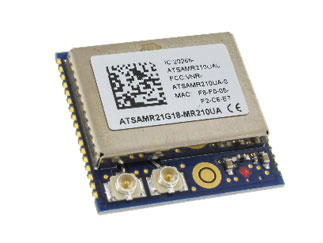
\includegraphics[width=0.35\textwidth,keepaspectratio]{figures/samr21}
	\caption{SAM R21 Xplained Pro module.}

\end{figure}

%%%%%%%%%%%%%%%%%%%%%%%%%%%%%%%

\subsection{CC1310 SimpleLink™ Sub-1 GHz Ultra-Low Power Wireless Microcontroller}

\begin{framed}
	
	http://www.ti.com/product/CC1310
	
	\vspace{1em}
	\hline
	\vspace{1em}
\small	
	\textit{The CC1310 is a member of the CC26xx and CC13xx family of cost-effective, ultra-low-power, 2.4-GHz and Sub-1 GHz RF devices. Very low active RF and microcontroller (MCU) current consumption, in addition to flexible low-power modes, provide excellent battery lifetime and allow long-range operation on small coin-cell batteries and in energy-harvesting applications.}
		
	\textit{The CC1310 device is the first device in a Sub-1 GHz family of cost-effective, ultra-low-power wireless MCUs. The CC1310 device combines a flexible, very low power RF transceiver with a powerful 48-MHz Cortex®-M3 microcontroller in a platform supporting multiple physical layers and RF standards. A dedicated Radio Controller (Cortex®-M0) handles low-level RF protocol commands that are stored in ROM or RAM, thus ensuring ultra-low power and flexibility. The low-power consumption of the CC1310 device does not come at the expense of RF performance; the CC1310 device has excellent sensitivity and robustness (selectivity and blocking) performance.}
		
\end{framed}




\vspace{-1.5em}
\begin{figure}[h!]
	\centering
	\begin{minipage}{.5\textwidth}
		\centering
		\vspace{2.5em}
		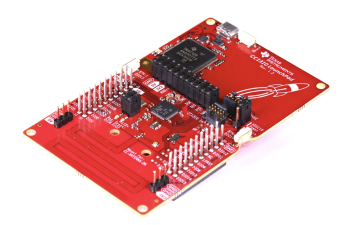
\includegraphics[width=1\textwidth,keepaspectratio]{figures/cc1310_board}
		\vspace{2em}
		\captionof{figure}{CC1310 evaluation board.}
		\label{fig:test1}
	\end{minipage}%
	\begin{minipage}{.5\textwidth}
		\centering
		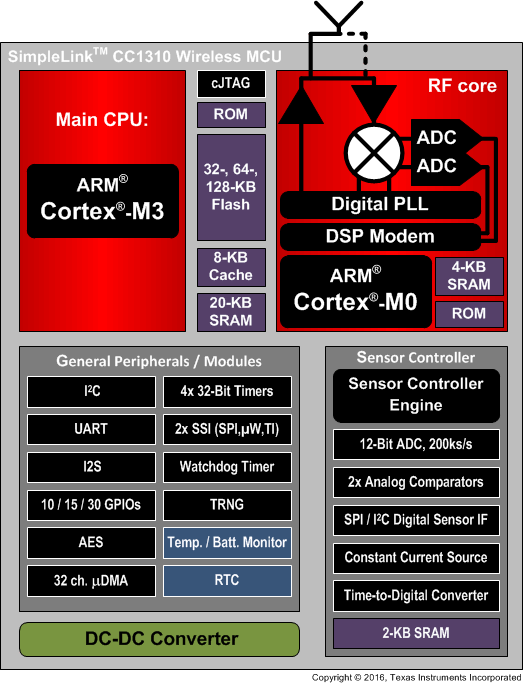
\includegraphics[width=0.70\textwidth,keepaspectratio]{figures/cc1310}
		\captionof{figure}{CC1310 chip architecture.}
		\label{fig:test2}
	\end{minipage}
\end{figure}
The CC1310 is a Texas Instruments platform launched to operate the sub-GHz frequency band. It depends on a ARM® Cortex®-M3 processor and an integrated ultra-low-power RF Core. It is integrated in the category of "Wireless MCU's" due to it's integration of CPU and RF core, similarly to the Atmel SAM-R21 previoulsy presented platform.


%%%%%%%%%%%%%%%%%%%%%%%%%%%

\subsection{Adafruit Feather 32u4 Radio (RFM69HCW)}

\begin{framed}
	
	https://learn.adafruit.com/adafruit-feather-32u4-radio-with-rfm69hcw-module/overview
	
	\vspace{1em}
	\hline
	\vspace{1em}
\small	
	\textit{This Adafruit Feather 32u4 Radio (RFM69HCW) 900MHz microcontroller packet radio transceiver with built in USB and battery charging. 32u4 with a 900MHz radio module cooked in an Adafruit Feather. Great for making wireless networks that can go further than 2.4GHz 802.15.4 and similar, are more flexible than Bluetooth LE and without the high power requirements of WiFi. The 900MHz radio version can be used for either 868MHz or 915MHz transmission/reception. At the Feather, 32u4's heart is at ATmega32u4 clocked at 8MHz and at 3.3V logic. This chip has 32K of flash and 2K of RAM, with built in USB so not only does it have a USB-to-Serial program and debug capability built in with no need for an FTDI-like chip, it can also act like a mouse, keyboard, USB MIDI device, etc.}
\end{framed}

%%%%%%%%%%%%%%%%%%%%%%%%%%%

\subsection{Adafruit Feather HUZZAH ESP8266}

\begin{framed}
	
	https://learn.adafruit.com/adafruit-feather-huzzah-esp8266/overview
	
	\vspace{1em}
	\hline
	\vspace{1em}
\small	
	\textit{This is the Adafruit Feather HUZZAH ESP8266 - our take on an 'all-in-one' ESP8266 WiFi development board with built in USB and battery charging. At the Feather HUZZAH's heart is an ESP8266 WiFi microcontroller clocked at 80 MHz and at 3.3V logic. This microcontroller contains a Tensilica chip core as well as a full WiFi stack. You can program the microcontroller using the Arduino IDE for an easy-to-run Internet of Things core. We wired up a high-quality SiLabs CP2104 USB-Serial chip that can upload code at a blistering 921600 baud for fast development time. It also has auto-reset so no noodling with pins and reset button pressings. The CP2104 has better driver support than the CH340 and can do very high speeds without stability issues.}
\end{framed}

%%%%%%%%%%%%%%%%%%%%%%%%%%%

\vspace{-1em}
\begin{figure}[h!]
	\centering
	\begin{minipage}{.47\textwidth}
		\centering

		\includegraphics[width=0.90\textwidth,keepaspectratio]{figures/feather_3077}

		\captionof{figure}{Adafruit Feather 32u4 Radio (RFM69HCW).}
		\label{fig:test3}
	\end{minipage}%
	\begin{minipage}{.05\textwidth}
		\centering
		~
	\end{minipage}%	
	\begin{minipage}{.47\textwidth}
		\centering
		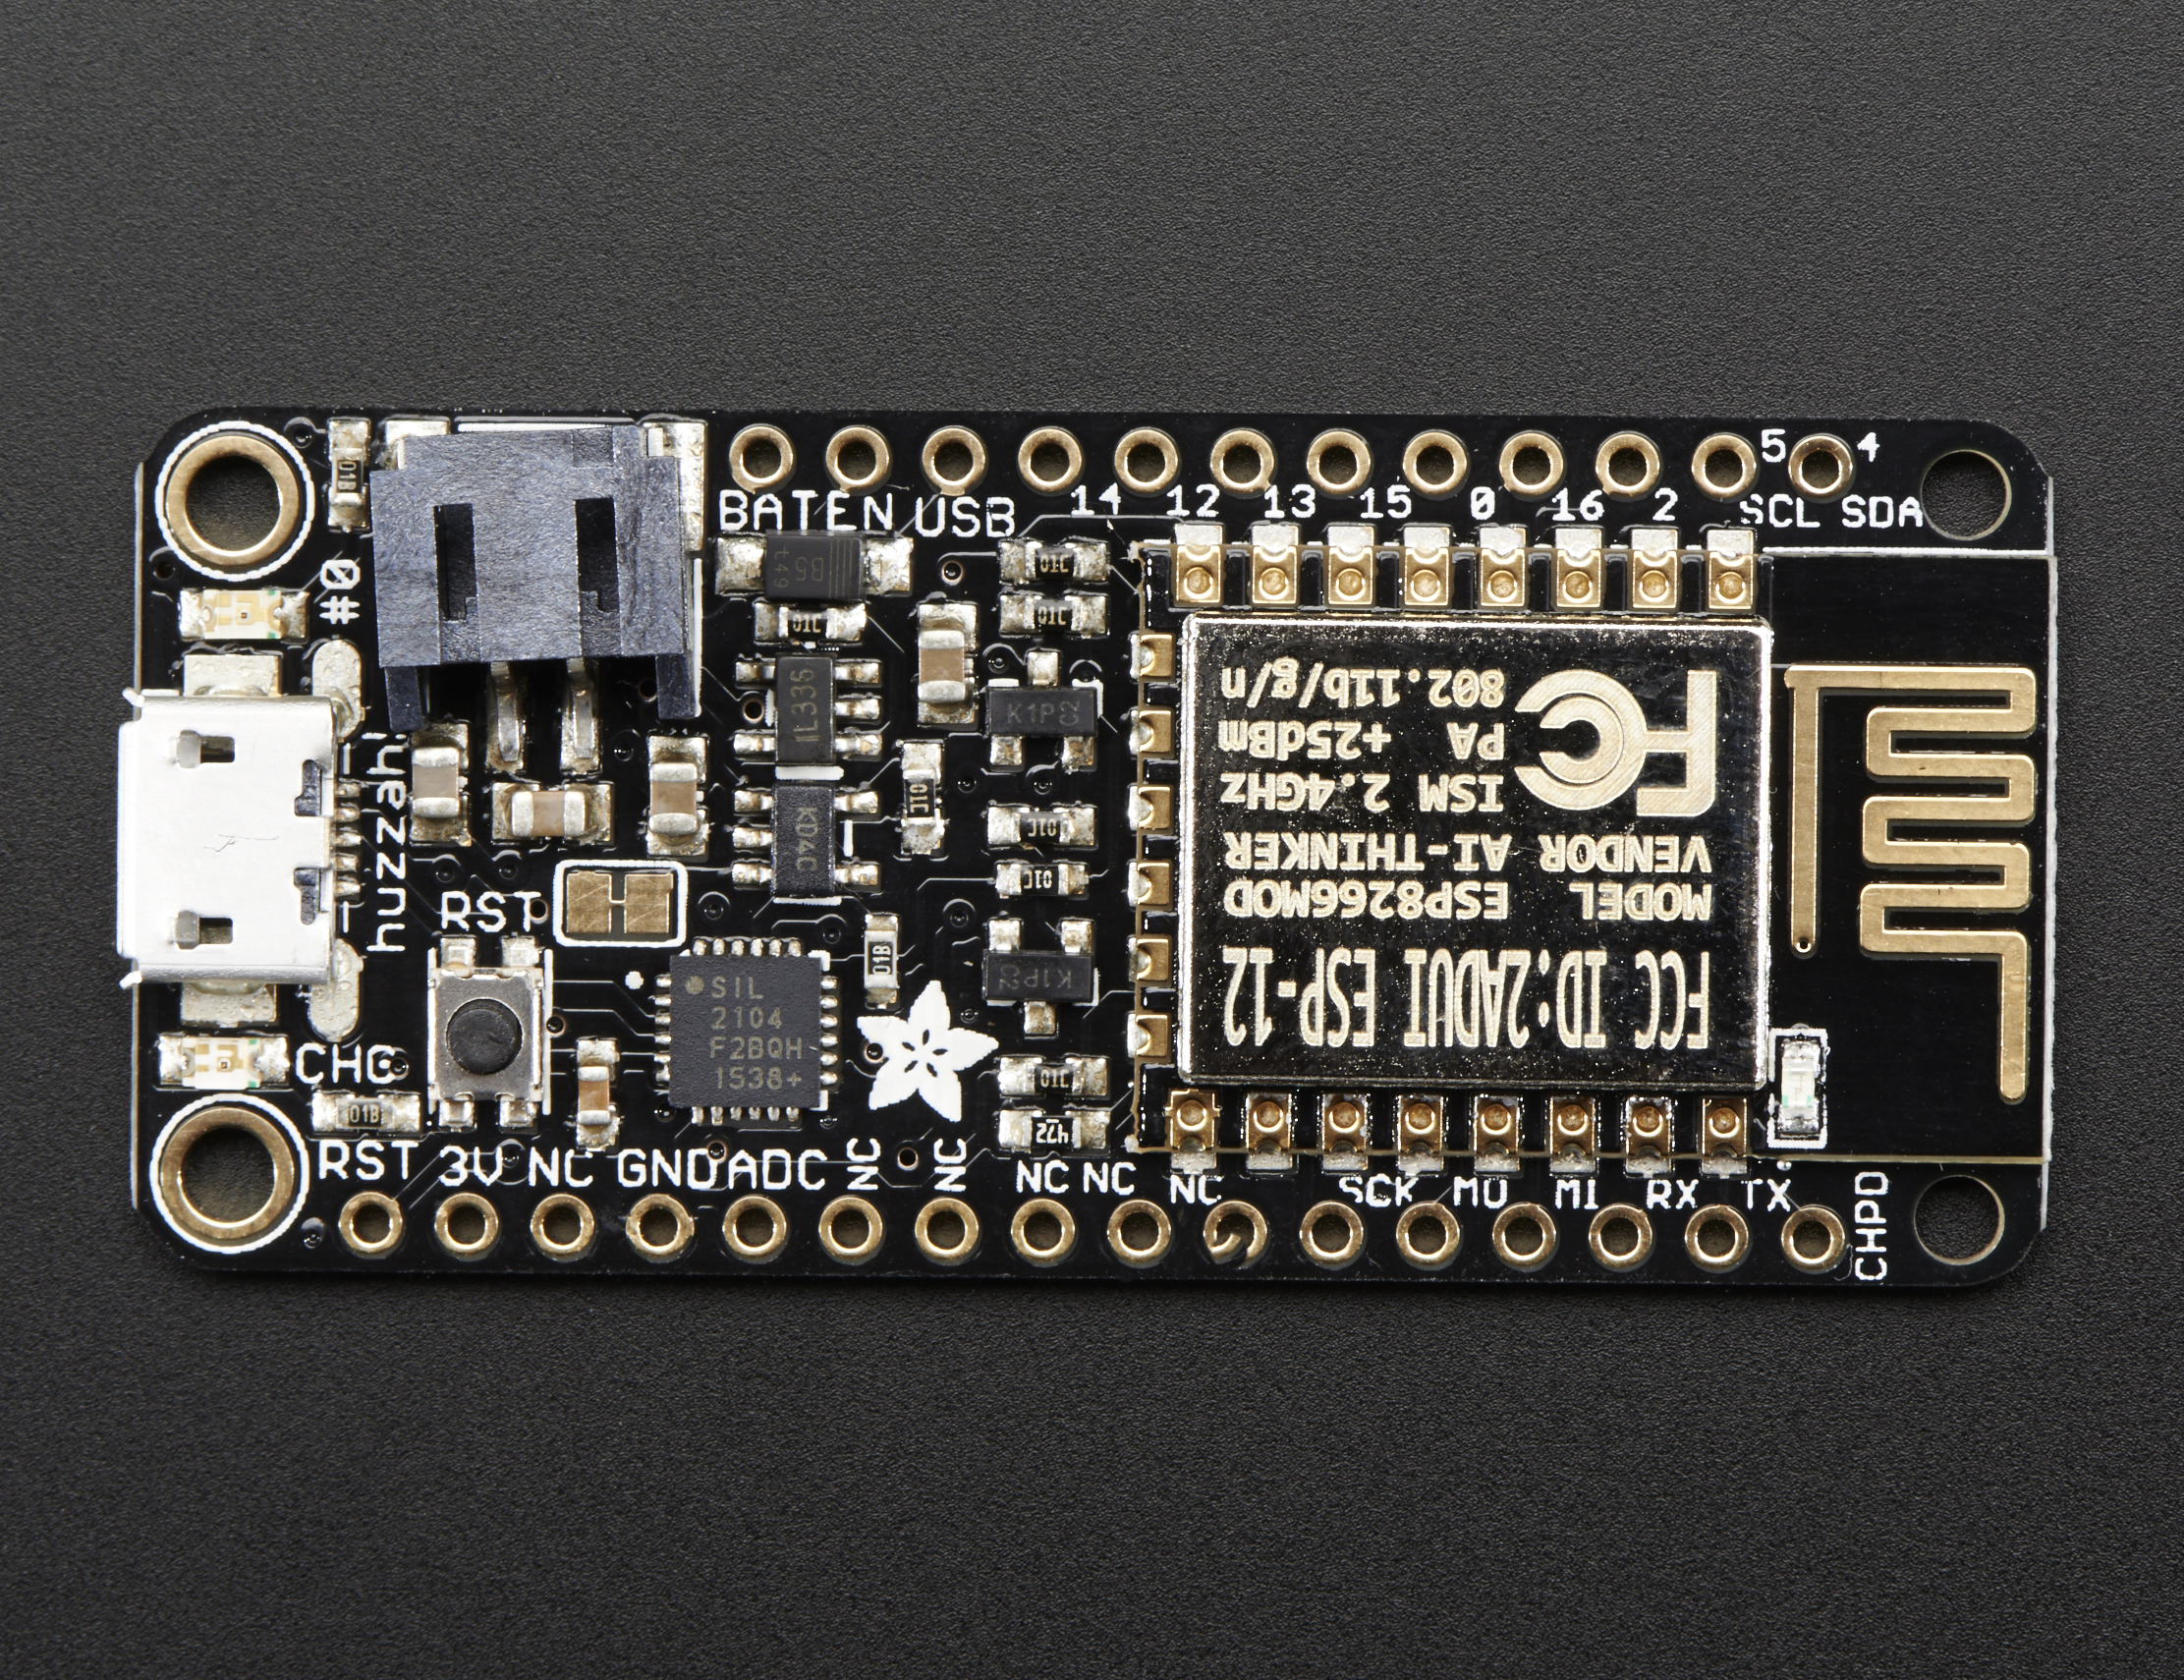
\includegraphics[width=0.90\textwidth,keepaspectratio]{figures/feather_wifi}
		\captionof{figure}{Adafruit Feather HUZZAH ESP8266.}
		\label{fig:test4}
	\end{minipage}
\end{figure}

Both Adafruit Feather modules (for sub-GHz and for WiFi) are designed for cheap and modular solutions.

\subsection{ATxmega256A3U AT86RF233 ZigBit Module}

\begin{framed}
	
	http://www.atmel.com/pt/br/devices/ATxmega256A3U-and-AT86RF233-ZigBit-Wireless-Module.aspx
	
	\vspace{1em}
	\hline
	\vspace{1em}
\small	
	\textit{The Atmel ZigBit 2.4GHz ATZB-X0-256-3-0-C wireless system-on-module is designed to work with IEEE 802.15.4 and ZigBee WPAN communication protocols. The ZigBit module is compatible with a ZigBee stack that supports a self-healing, self-organizing mesh network, while optimizing network traffic and minimizing power consumption.}
\end{framed}

\begin{figure}[h!]
	\centering
	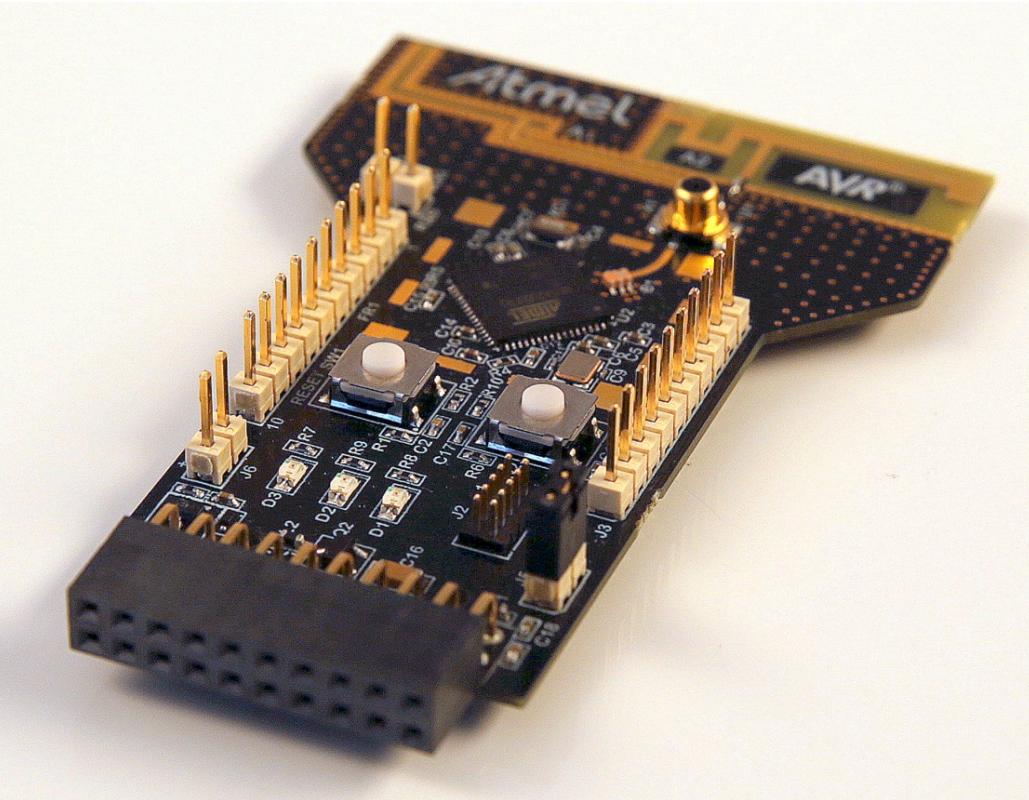
\includegraphics[width=0.35\textwidth,keepaspectratio]{figures/atxmega}
	\caption{ATxmega256A3U AT86RF233 ZigBit Module.}
	
\end{figure}

%%%%%%%%%%%%%%%%%%%%%%%%%%

\subsection{CC1350 SimpleLink™ Ultra-Low Power Dual Band Wireless Microcontroller}

\begin{framed}
	
	http://www.atmel.com/pt/br/devices/ATxmega256A3U-and-AT86RF233-ZigBit-Wireless-Module.aspx
	
	\vspace{1em}
	\hline
	\vspace{1em}
\small	
	\textit{The CC1350 is a member of the CC26xx and CC13xx family of cost-effective, ultra-low-power, 2.4-GHz and Sub-1 GHz RF devices from Texas Instruments™. Very low active RF and microcontroller (MCU) current consumption, in addition to flexible low-power modes, provide excellent battery lifetime and allow long-range operation on small coin-cell batteries and in energy-harvesting applications.}
		
		\textit{The CC1350 is the first device in the CC13xx and CC26xx family of cost-effective, ultra-low-power wireless MCUs capable of handling both Sub-1 GHz and 2.4-GHz RF frequencies. The CC1350 device combines a flexible, very low-power RF transceiver with a powerful 48-MHz ARM® Cortex®-M3 microcontroller in a platform supporting multiple physical layers and RF standards. A dedicated Radio Controller (Cortex®-M0) handles low-level RF protocol commands that are stored in ROM or RAM, thus ensuring ultra-low power and flexibility to handle both Sub-1 GHz protocols and 2.4 GHz protocols (for example Bluetooth® low energy). This enables the combination of a Sub-1 GHz communication solution that offers the best possible RF range together with a Bluetooth low energy smartphone connection that enables great user experience through a phone application. The Sub-1 GHz only device in this family is the CC1310.}
\end{framed}

This CC1350 adds the Bluetooth® low energy functionality to the CC1310 module with small increase on the cost of the solution. 

\section{Protocols and standards}
\lipsum[4]

\section{Communication KPI’s}
\lipsum[4]

\chapter{Development of Wireless Monitoring System}
%\lipsum[4-4]
In this chapter is presented the development of the wireless monitoring system, following the specifications and requirements raised in the chapter 2. This chapter is divided in four parts, starting with the description of the selected wireless technology. In \ref{sec:3.2} and \ref{sec:3.3} is presented the hardware and software architecture of the system. Communication results and KPI metrics are presented in section \ref{sec:3.4}. In section \ref{sec:3.5} is made the discussion of the results.

\section{Description of the selected wireless technology}
\label{sec:3.1}
%\lipsum[4-4]

The CC1350 platform was selected to fulfill the wireless requirements. The availability of Sub-1 GHz and Bluetooth technologies in the same device allows enough flexibility in terms of possible functionalities to be implemented. The powerful 32-bit ARM Cortex-M3 allows the implementation of a Real-time Operating System, capable of handling several tasks.

\section{Hardware architecture}
\label{sec:3.2}
%\lipsum[4-4]

The hardware architecture depends on serial communication between the power converter and the wireless node. Complementary, it depends on serial communication between the concentrator and the end user applications (serial monitor, Raspberry Pi and concentrator LCD). Figure \ref{fig:3.2.hw} presents the hardware architecture.

\begin{figure}[h!]
	\centering
	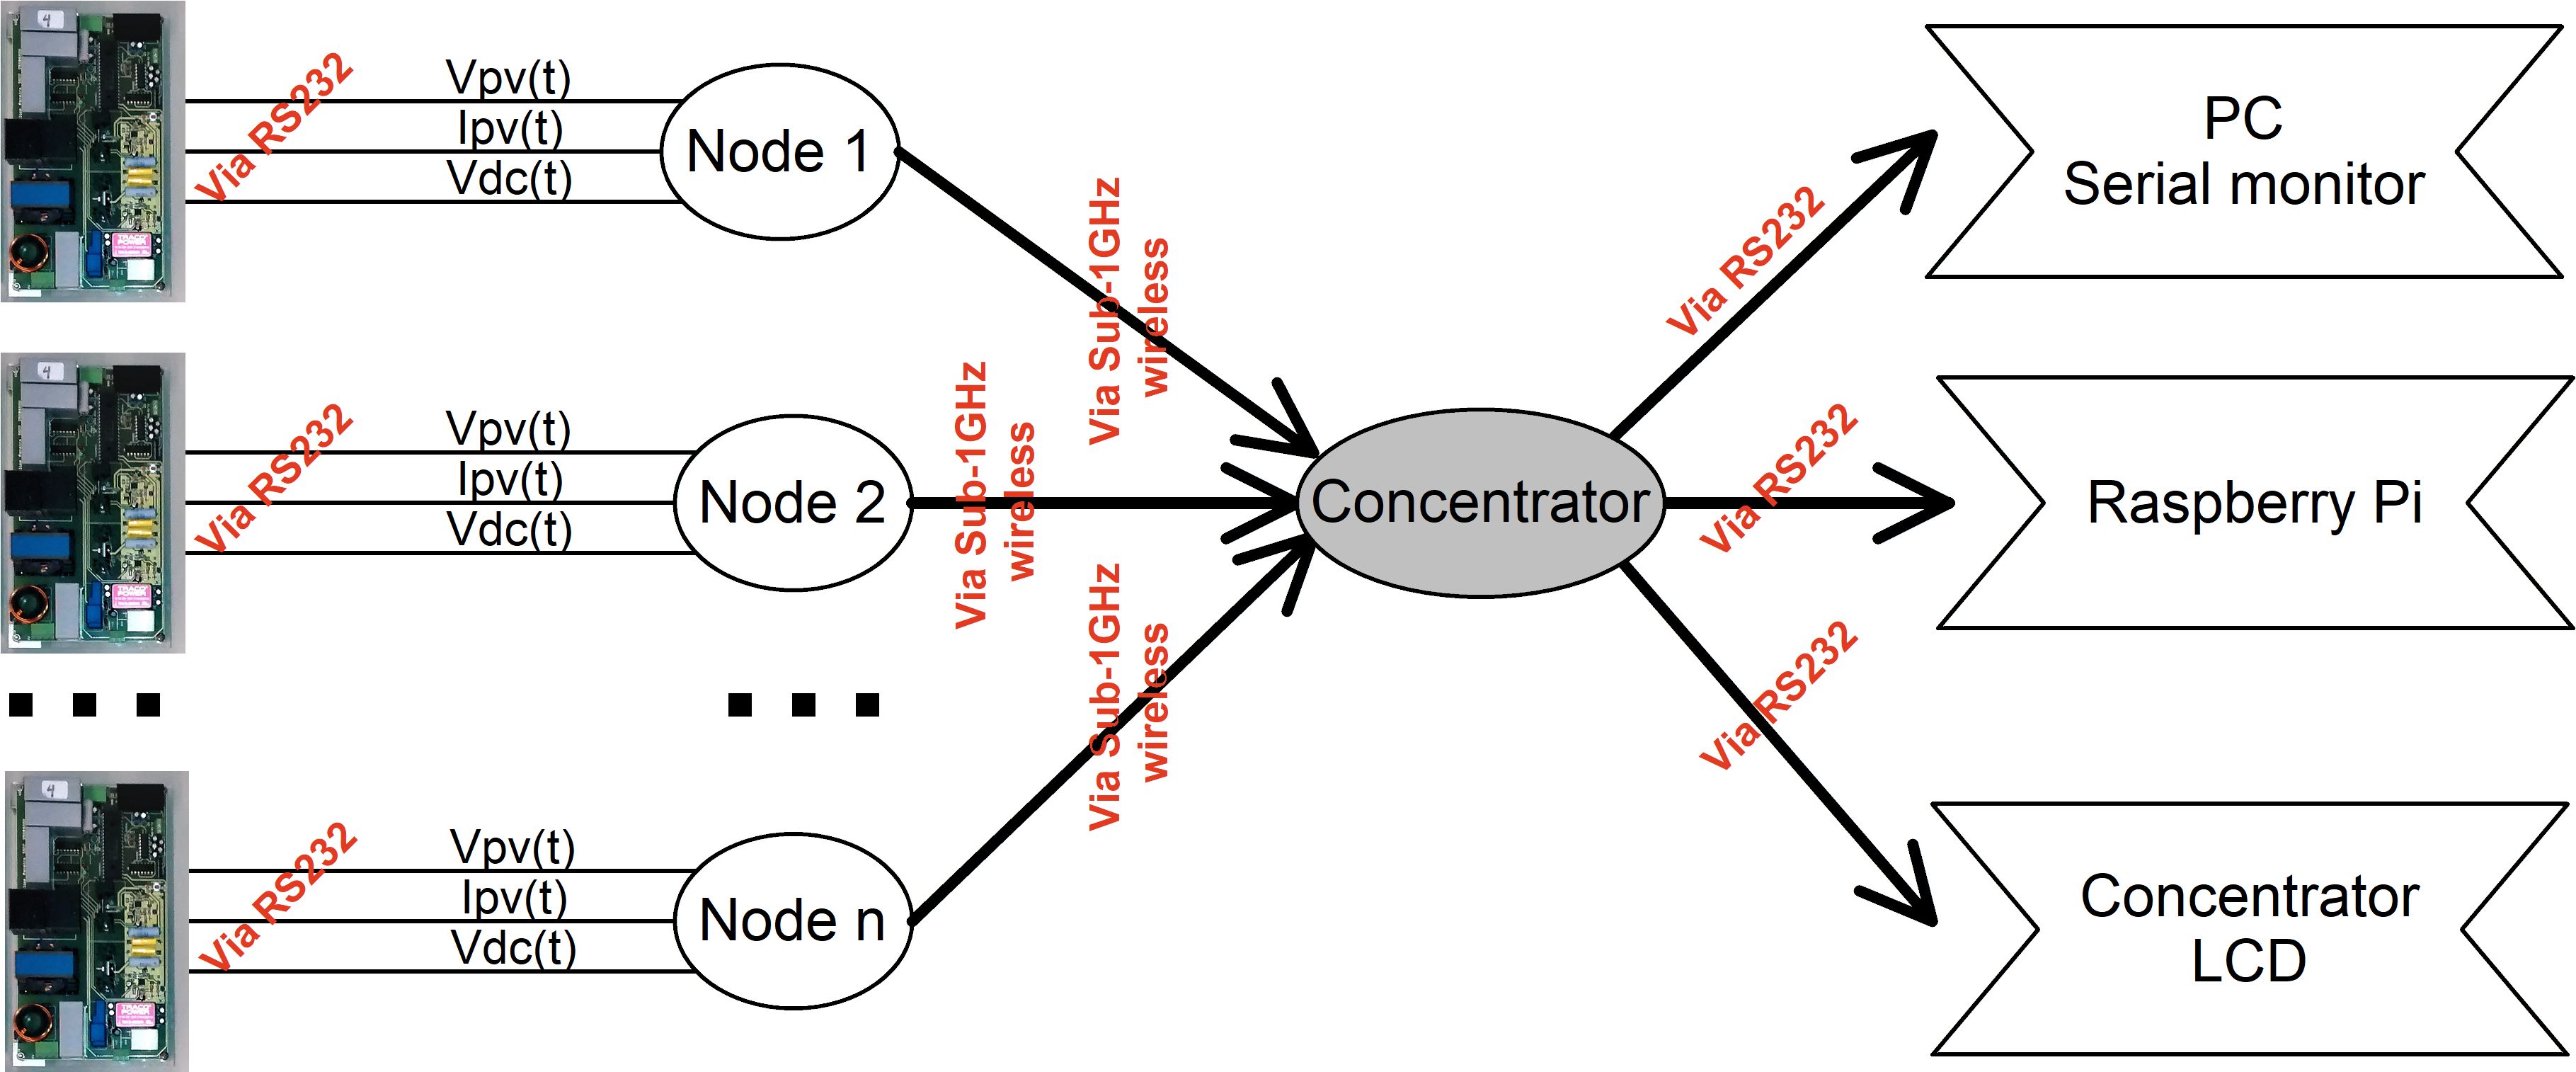
\includegraphics[width=0.9\textwidth,keepaspectratio]{figures/hw}
	\caption{Hardware architecture.}
	\label{fig:3.2.hw}
\end{figure}

The communication interface between node and power converter must support different voltage levels (in particular 3.3V from CC1350 node and 5V from power converter). This way, an electronic board (PCB) was developed to support this constraint. Complementary, this PCB allows a robust mechanical interface between the wireless node and the power converter, without extending the dimensions defined in the SRS. This PCB integration with wireless node and the power converter is presented in the figure \ref{fig:3.2.pcb}.

\begin{figure}[h!]
	\centering
	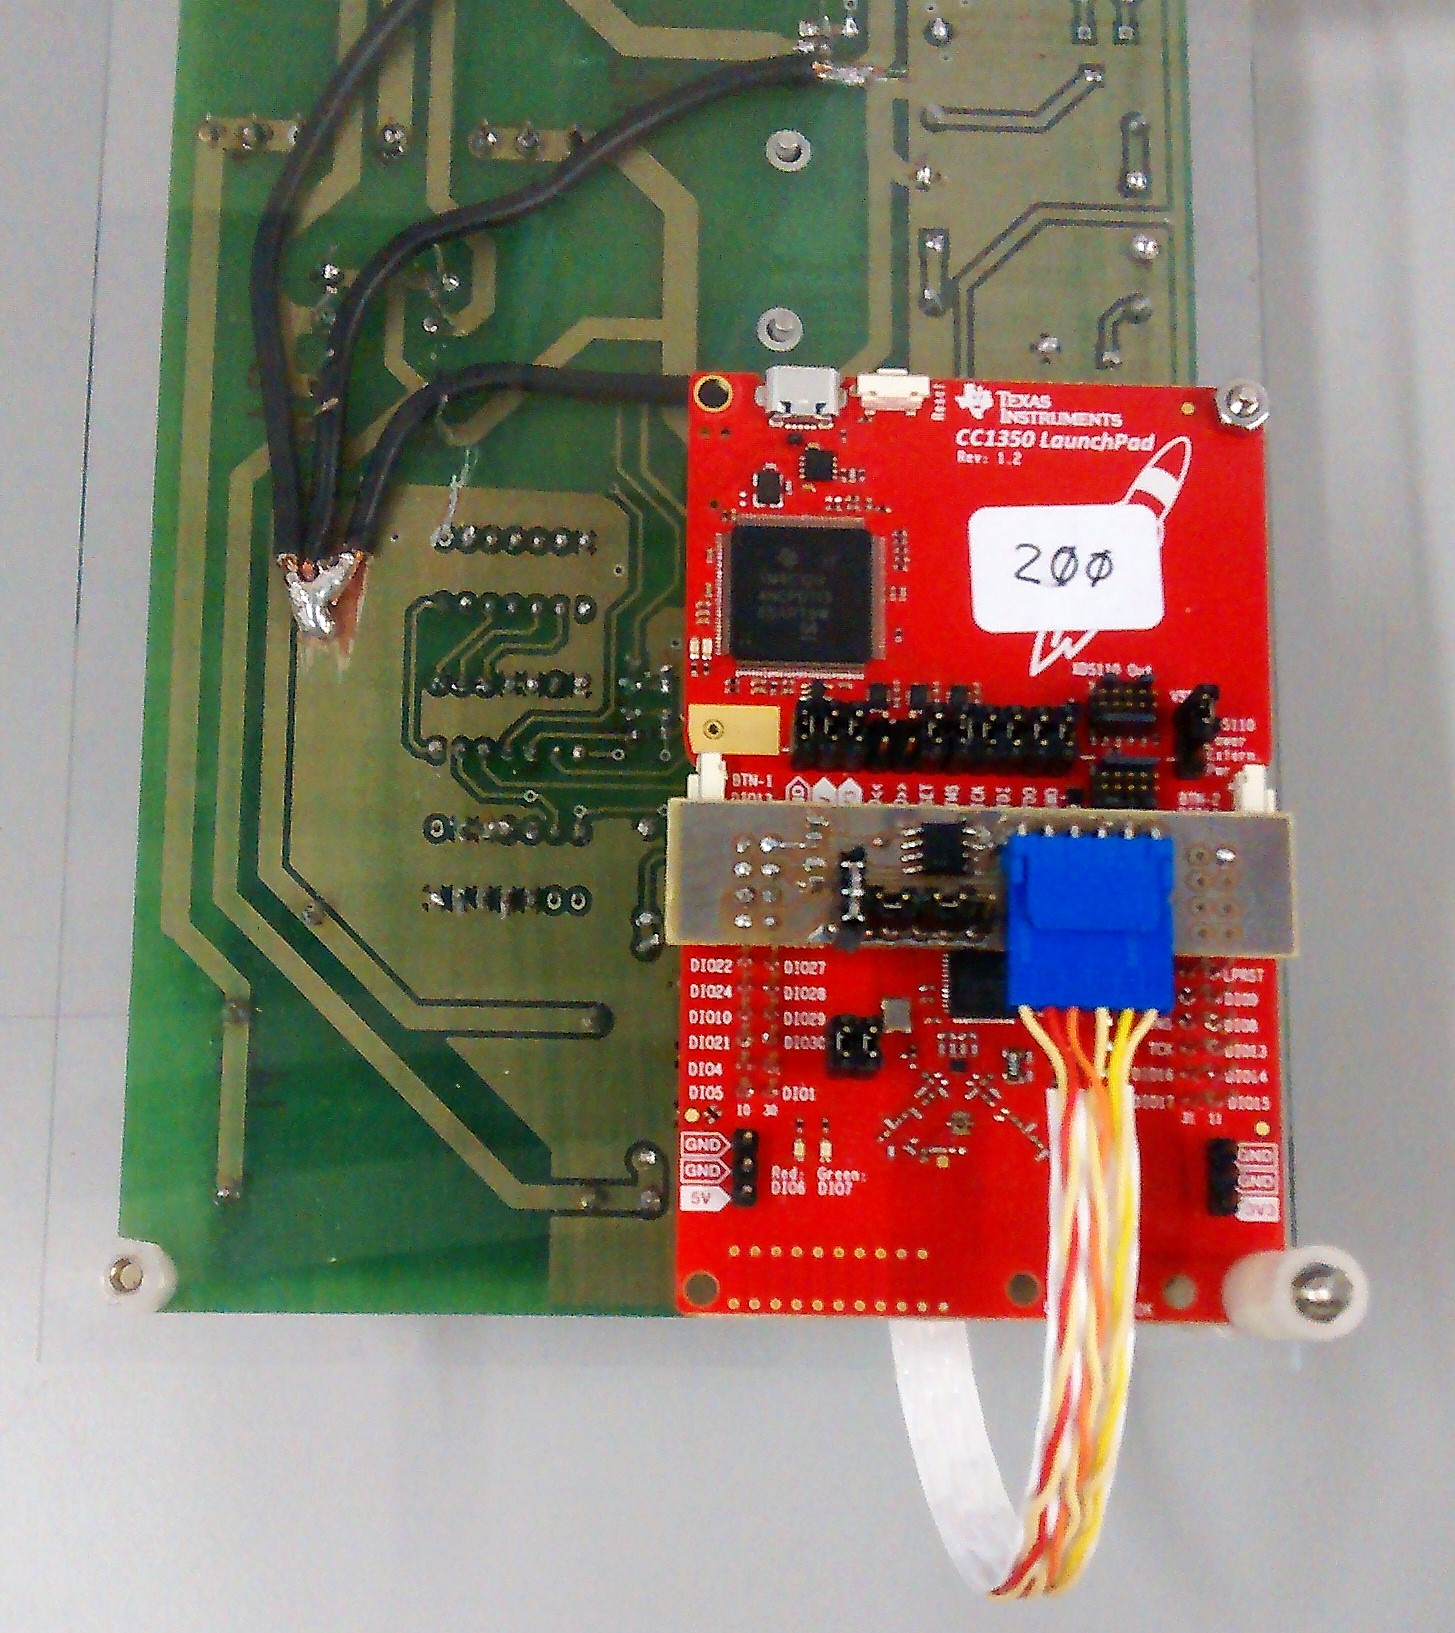
\includegraphics[width=0.4\textwidth,keepaspectratio]{figures/pcb}
	\caption{PCB integration with wireless node and the power converter.}
	\label{fig:3.2.pcb}
\end{figure}

On the concentrator side, the CC1350 development board has available the USB serial communication as well as the LCD as shown in figure \ref{fig:3.2.concentr}.

\begin{figure}[h!]
	\centering
	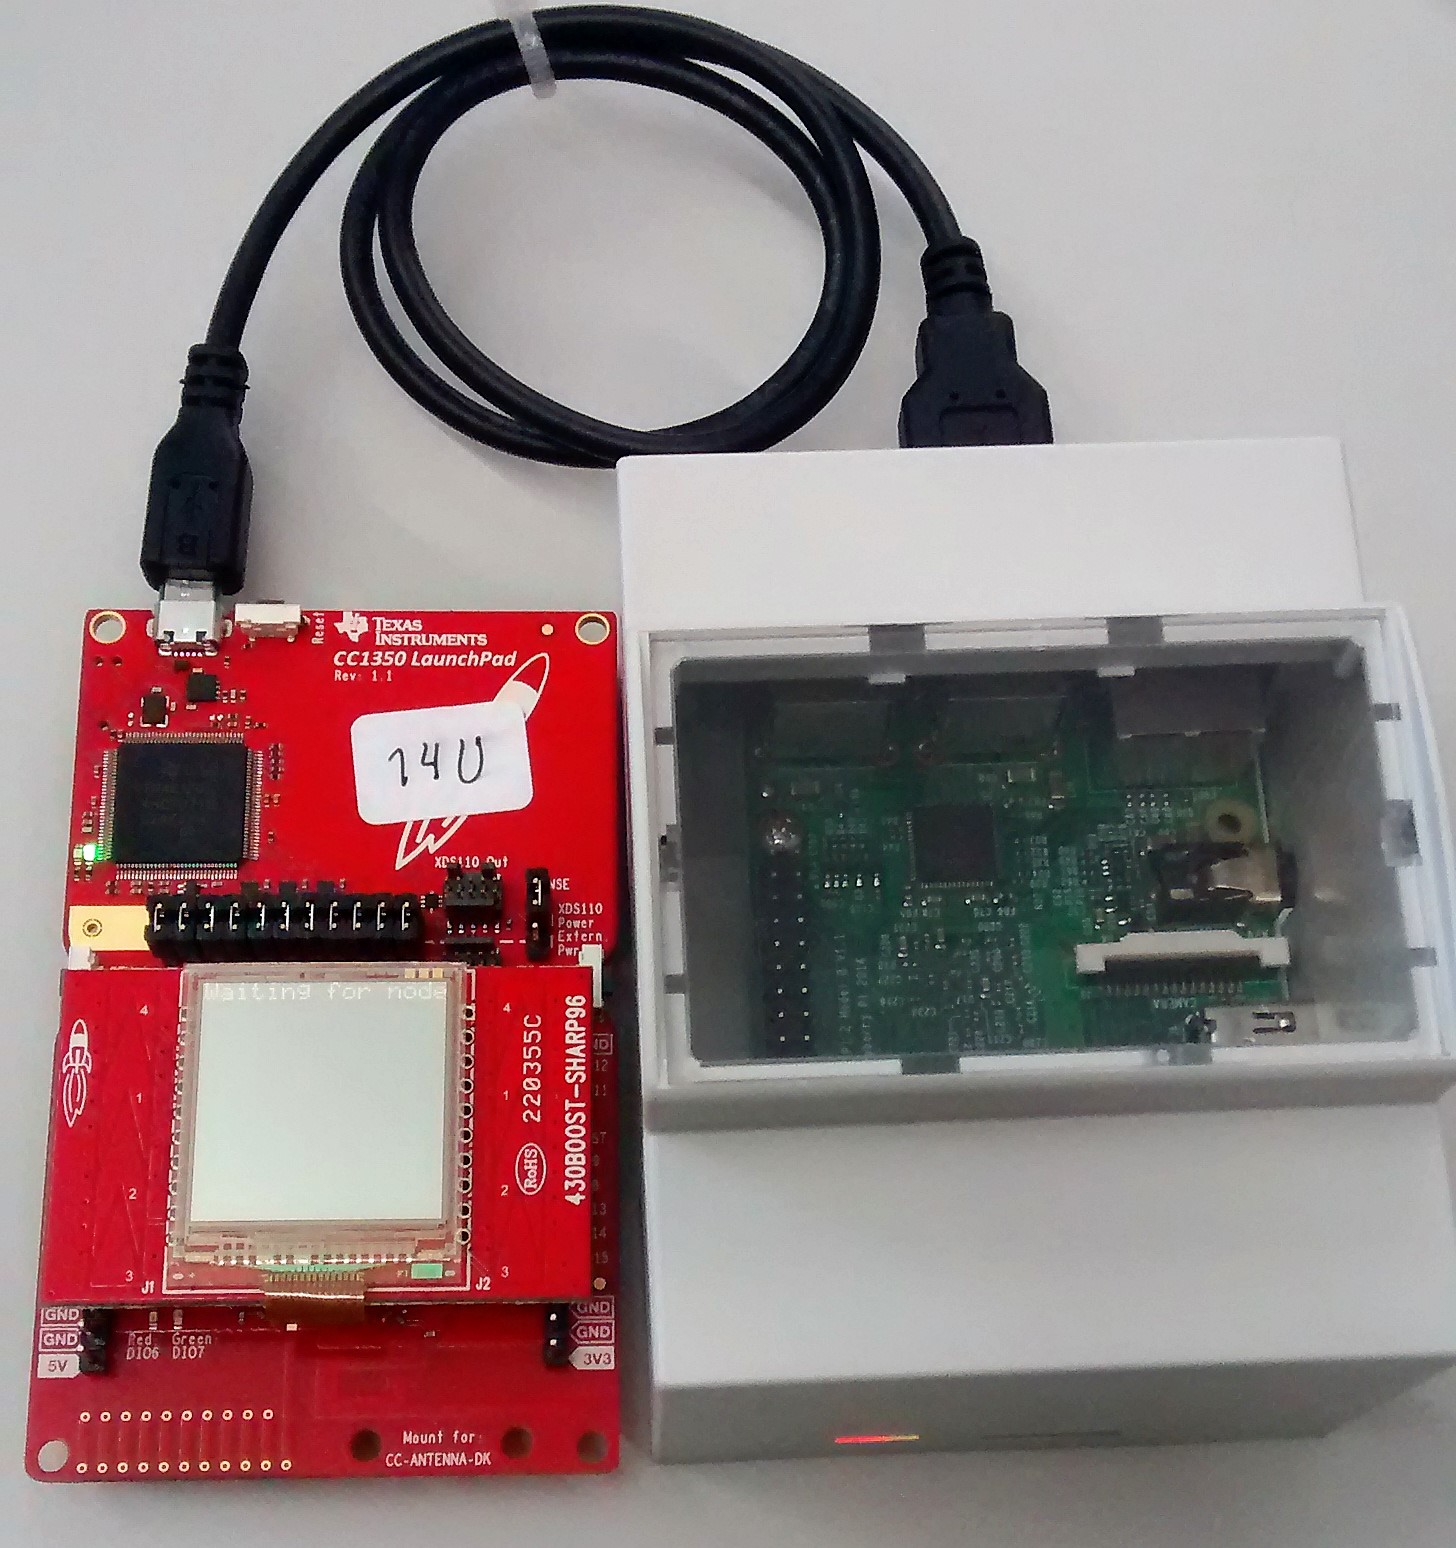
\includegraphics[width=0.5\textwidth,keepaspectratio]{figures/concentr}
	\caption{Concentrator connected to RPI.}
	\label{fig:3.2.concentr}
\end{figure}

\section{Software Architecture}
\label{sec:3.3}
%\lipsum[4-4]

As proposed in the SRS, figure \ref{fig:3.3.domainModel} presents the domain model of the software to be implemented in the concentrator and nodes.

\begin{figure}[h!]
	\centering
	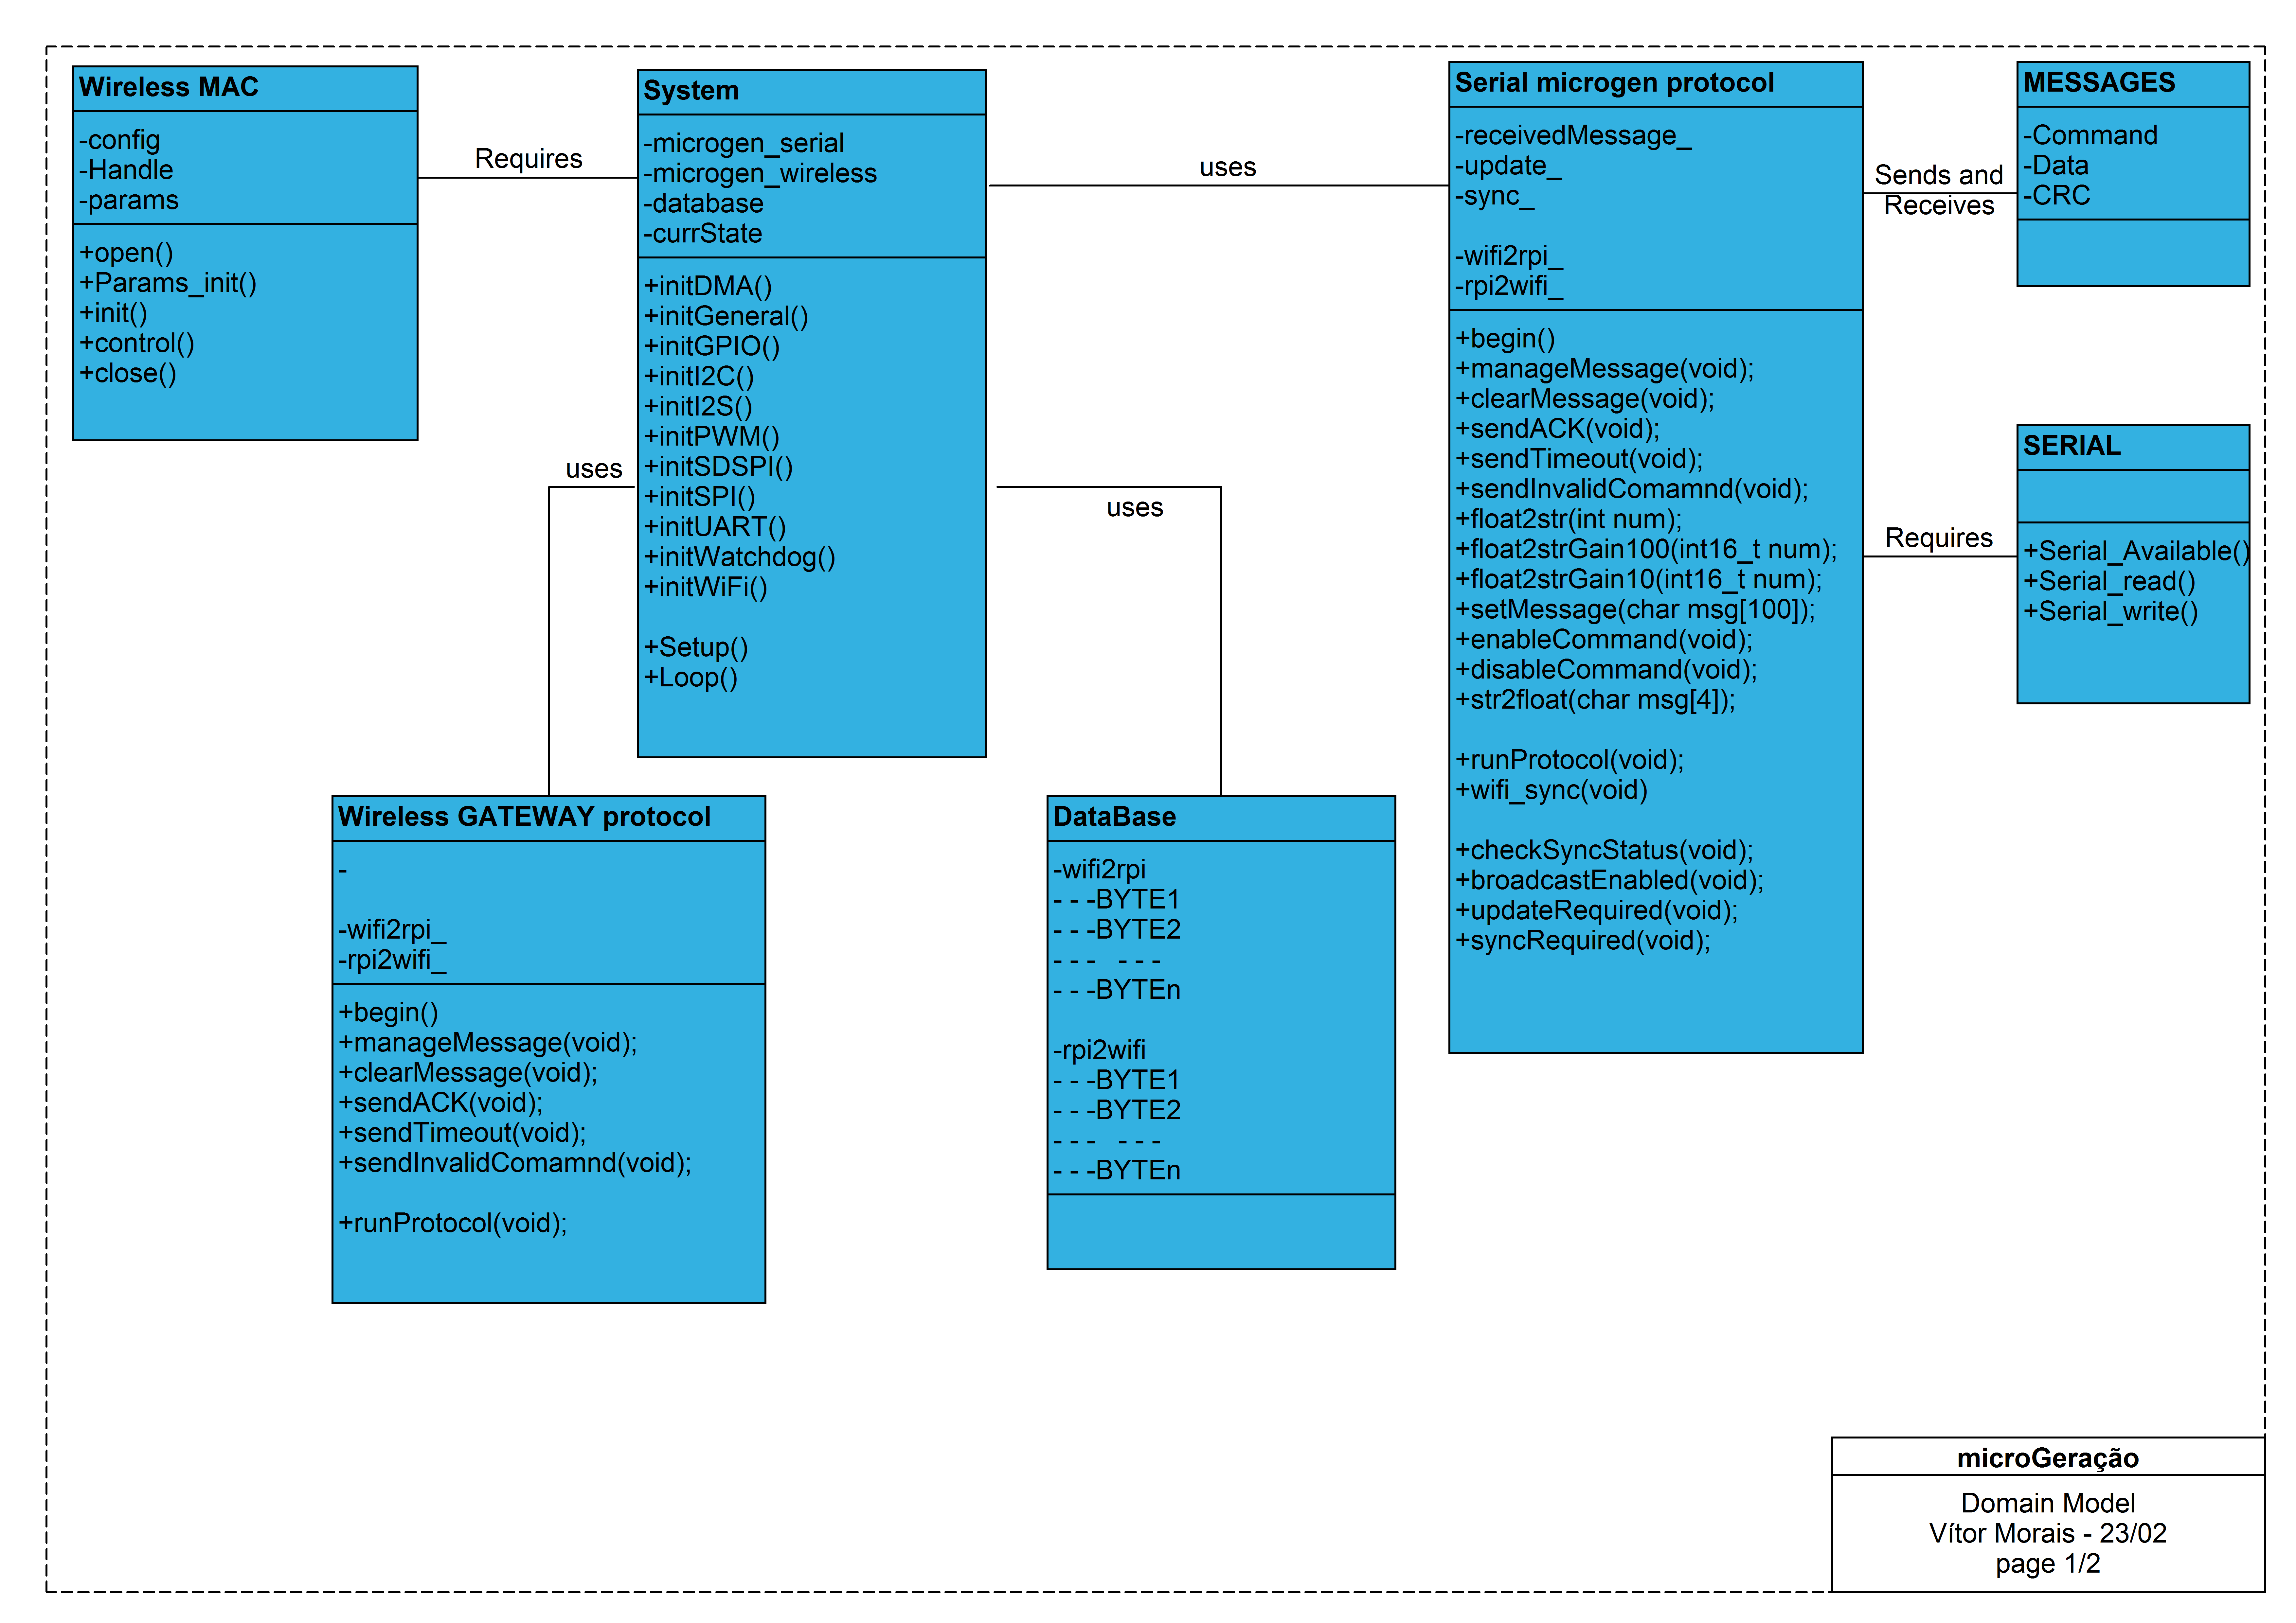
\includegraphics[width=\textwidth,keepaspectratio]{figures/domainModel}
	\caption{Domain Model Diagram.}
	\label{fig:3.3.domainModel}
\end{figure}

The software architecture was based on a proprietary implementation of a WSN by the manufacturer of the CC1350 (Texas Instruments).



\section{Communication results and KPI metrics}
\label{sec:3.4}
\lipsum[4-4]

\section{Discussion of the results}
\label{sec:3.5}
\lipsum[4-4]

%\chapter{Results and Discussion}
%\lipsum[4-4]

\chapter{Conclusions and Future Work}
%\lipsum[1]

With this work, we propose and implement a solution for the wireless monitoring of power converters. The main challenge of this wireless monitoring is to obtain energy data of a system in a harsh environment. The motivation for this work is to study the implementation of a wireless monitoring system in railway environment, based on the outcomes of the implementation of such monitoring system in a renewable energy generation system.

The system specification was defined, with the construction of a System Requirement Specification (SRS) document as the main outcome. In addition, it was performed an overview on existing wireless communication systems, a market survey on available technologies, and the protocols, standards and communication KPI's was raised.

A specific technology was selected, on the family of wireless MCU's. The implementation stage complies with the definition of the hardware and software architecture. The communication results validates the acquisition of electric measurements from multiple PV power converters. 

The lack of data results is clear. Any of the communication KPI's was not evaluated due to the need of further development. This further development depends on a new solution for the interface between the power converter and the wireless node, since the communication link is highly affected by the noise of power converter.

For future work is clear the need of evaluating all the proposed communication KPI's. This task requires a new electronic board to interface the remote node. Complementary, the data concentrator should be improved to implement a local database and a serial request-response protocol to exchange data with the microgeneration system master.

We conclude that the methodology followed and the proposed solution validates the objective of this work, which is the wireless monitoring of a power converter.



\bibliographystyle{chicago}
%chicago}

\bibliography{outliers,shift2rail,references}
%\bibliography{outliers}
%\PrintBib{outliers, }


%\bibliographystyle{plainnat}
%\bibliography{references}

\chapter*{Attachment 1 --- \large{Overview of communication systems for Smart Grids}}

\includepdf[pages=-, scale=0.9, offset=-10 0, pagecommand={\thispagestyle{plain}}]  {chapters/communication}
\chapter*{Attachment 2 --- \large{System Requirements Specification}}
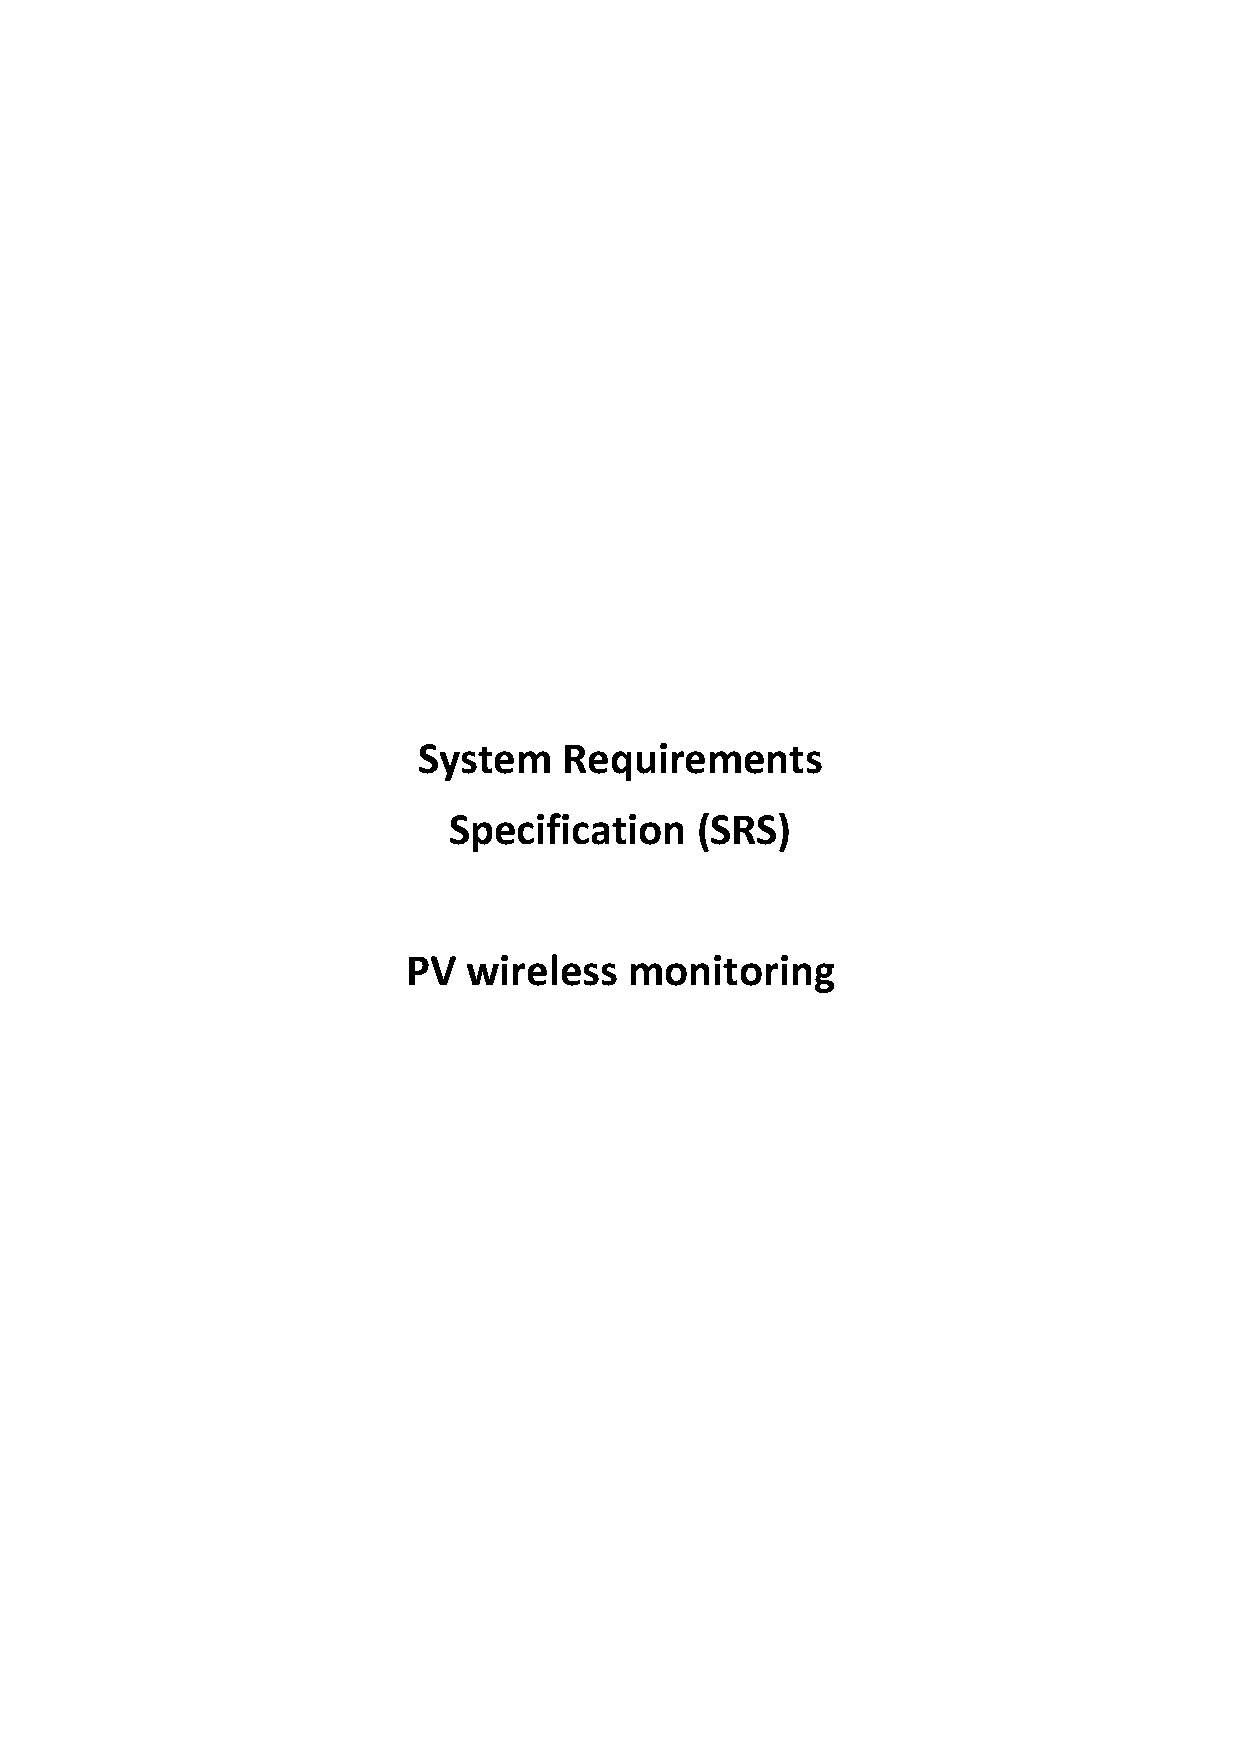
\includepdf[pages=-, scale=1, offset=0 0, pagecommand={\thispagestyle{plain}}]  {chapters/SRS}


\end{document}